\documentclass{article}
\usepackage{tikz}
\usepackage{amsmath}
\begin{document}

\title{Your Title}
\author{Your Name}
\date{\today} % You can set a specific date here

\maketitle
\begin{tikzpicture}
  % Draw the rectangular box
  \draw (0,0) rectangle (4,3);
  \draw[dashed] (0,3) rectangle (4,6);
  \draw[dashed] (4,3) rectangle (8,6);
  \draw[dashed] (4,0) rectangle (8,3);
  
  % Draw the point
  \fill (1,2) circle (2pt) node[above] {$s_0$};
  \fill (2,1) circle (2pt) node[above] {$t_0$};

  \fill (7,2) circle (1pt) node[above] {$s_1$};
  \fill (6,1) circle (1pt) node[above] {$t_1$};
  
  \fill (7, 4) circle (1pt) node[above] {$s_2$};
  \fill (6, 5) circle (1pt) node[above] {$t_2$};

  \fill (1,4) circle (1pt) node[above] {$s_3$};
  \fill (2,5) circle (1pt) node[above] {$t_3$};

\end{tikzpicture}





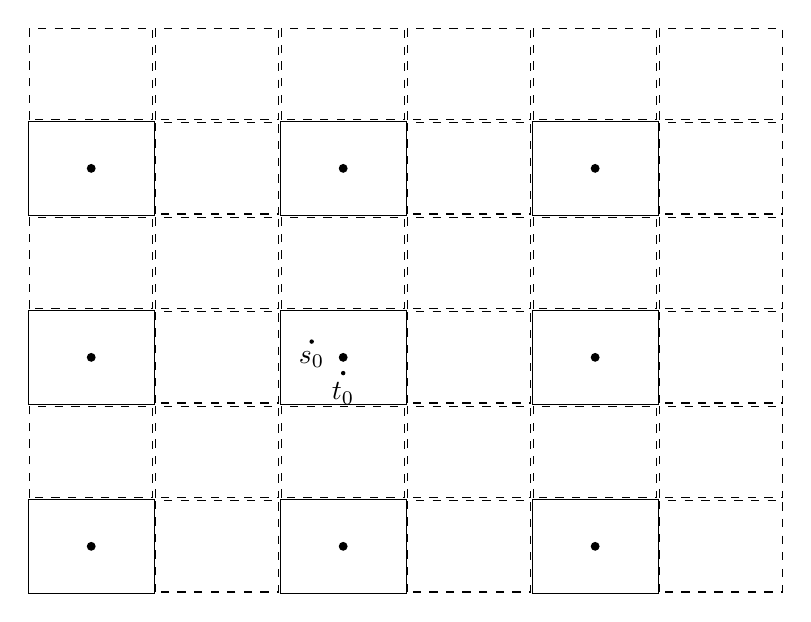
\begin{tikzpicture}[scale=0.4]
  
  % Draw the point
  \fill (1,2) circle (2pt) node[below] {$s_0$};
  \fill (2,1) circle (2pt) node[below] {$t_0$};

% Define the number of rows and columns in the grid
  \def\nRows{1}
  \def\nCols{1}
 
  \def\boxMargin{0.05}
  % Draw the grid of points
  \foreach \row in {-\nRows,...,\nRows} {
    \foreach \col in {-\nCols,...,\nCols} {
    	\draw (\row*2*4,  \col*2*3) rectangle (\row*2*4 + 4,  \col*2*3 + 3);
	  \draw[dashed] (\row*2*4 + 4 + \boxMargin,  \col*2*3 + \boxMargin) rectangle (\row*2*4 + 4 + 4 - \boxMargin,  \col*2*3 + 3 - \boxMargin) ;
	  \draw[dashed] (\row*2*4 + \boxMargin,  \col*2*3 + 3 + \boxMargin) rectangle  (\row*2*4 + 4 - \boxMargin,  \col*2*3 + 3 + 3 - \boxMargin);
	  \draw[dashed] (\row*2*4 + 4 + \boxMargin,  \col*2*3 + 3 +\boxMargin) rectangle (\row*2*4 + 4 + 4 - \boxMargin,  \col*2*3 + 3 + 3 - \boxMargin);
	  \fill (\row*2*4 + 2, \col*2*3 + 1.5) circle (4pt);
    }
  }


\end{tikzpicture}


\[
\Delta k_x =
\begin{cases}
 \left\lceil \frac{\Delta x}{2w\Delta_0 k_x} \right\rceil & \text{if } p(k_0) \text{ is not in the same direction as } v \\
 \\
 \left\lfloor \frac{\Delta x}{2w\Delta_0 k_x} \right\rfloor & \text{if } p(k_0) \text{ is in the same direction as } v 
\end{cases}
\]

\begin{tikzpicture}
  
  % Draw the point
  \fill (0, 0) circle (5pt) node[below,font=\LARGE] {$0$};
  
  \fill (2,1) circle (4pt) node[left,font=\LARGE] {$s$};
  \fill (5,8) circle (4pt) node[right,font=\LARGE] {$t$};
  
   \def\nRows{2}
  \def\nCols{2}
    \def\nRows{1}
  %\def\offx{2 + 3}
  %\def\offy{1 + 7}
  \def\offx{3.5}
  \def\offy{4.5}
 
  \fill (\offx - 6,\offy) circle (4pt) node[right,font=\LARGE] {$p_0$};
  
   \draw[->, thick] (\offx +3, \offy + 7) -- (\offx, \offy) node[pos=1, sloped, below,font=\LARGE] {$ \lfloor p(k) \rfloor $};
   \fill (\offx +3, \offy + 7) circle (2pt) node[left,font=\LARGE] {$p(k_0)$};
   \draw[->,  thick] (\offx +3, \offy + 7) -- (\offx - 3, \offy - 7) node[pos=1, sloped, below,font=\LARGE] {$\lceil p(k) \rceil $};
   
   \draw[<->, dashed] (2, 1) -- (\offx +3, 1) node[midway,below,font=\LARGE] {$\Delta x$};
   \draw[dashed]  (\offx +3, 1) -- (\offx +3, \offy + 7);

  \foreach \row in {-2,...,1} {
    \foreach \col in {-1,...,1} {
	  \fill (\offx + \row*2*1.5, \offy + \col*2*3.5) circle (4pt);
    }
  }

\end{tikzpicture}

\begin{tikzpicture} 
% Draw the rectangular box
\draw (0,0) rectangle (4,3);
% Draw the point
\fill (1,2) circle (2pt) node[above] {s};
% Define the slope of incidence
\pgfmathsetmacro{\slope}{30}
% Draw the incident ray
\draw (1,2) -- ++(\slope:2) coordinate (incident);
% Calculate the slope of reflection
\pgfmathsetmacro{\reflectslope}{0 - \slope}
% Calculate the reflection point
\path (incident) -- ++(\reflectslope:1) coordinate (reflection);
% Draw the reflected ray
\draw (incident) -- (reflection);
 \end{tikzpicture}
\begin{tikzpicture}
  % Draw the rectangular box
  \draw (0,0) rectangle (4,3);
  \draw (0,3) rectangle (4,6);
  
  % Draw the point
  \fill (1,2) circle (2pt) node[above] {s};
  
  \fill (1, 4) circle (2pt) node[above] {s'};
  
  % Define the slope of incidence
  \pgfmathsetmacro{\slope}{30}
  
  % Draw the incident ray
  \draw (1,2) -- ++(\slope:3) coordinate (incident);
  
\end{tikzpicture}

\end{document}